
\documentclass[leqno]{article}
\usepackage[top=10em]{geometry}
\usepackage{amsmath}
\usepackage{tikz}
\usepackage{tikz-qtree,tikz-qtree-compat}
\usepackage{graphicx}
\usepackage[margin=1cm]{caption}
\usepackage{paralist}
\usepackage{wrapfig}
\usepackage[colorlinks, linkcolor=purple]{hyperref}
\usepackage{cleveref}

\title{Compressive Saliency Sensing: sampling near the edges}
\date{}
\author{Scott Sievert\\ \texttt{sieve121@umn.edu}}

\newcommand{\kron}{http://en.wikipedia.org/wiki/Kronecker\_product\#Matrix\_equations}

\begin{document}


    \maketitle
    {\hypersetup{linkcolor=blue} \tableofcontents}
    \hrulefill

    \section{One Dimension}
        In one dimension, we do not have a tree like we do in the two dimension case. Instead of having three branches like the 2D case, we have two branches at each node.

        \subsection{Approximating the Wavelet transform}

          
          Lets say we have an $n$ dimensional signal: $x = (x_1,\ldots,x_n)^T$. We can take the wavelet transform of this signal, $w$, using $x = h w$, where $h$ is the wavelet matrix (in our case, the simple Haar matrix).


            The terms in $w$ correspond to different frequency components, and the latter terms correspond to higher frequencies. We only care about these terms if we're close to an edge, since that's where high frequency terms are. There's no need to approximate a DC or constant term with high frequency.

            So let's say we're only interested in the top $m$ terms of $w$, since what's specified when we approximate the wavelet. Since we only care about the upper portions of $w$, we can get rid of the corresponding rows for $h$.

            $$ 
                \begin{bmatrix}  
                    h_{1,1} & h_{1,2} &h_{1,3} &h_{1,4} \\
                    h_{2,1} & h_{2,2} &h_{2,3} &h_{2,4} \\
                    h_{3,1} & h_{3,2} &h_{3,3} &h_{3,4} \\
                    h_{4,1} & h_{4,2} &h_{4,3} &h_{4,4} \\
                
                \end{bmatrix}
                \begin{bmatrix}
                    w_1 \\ w_2 \\ w_3 \\ w_4
                \end{bmatrix}
            $$

            Since we only care about the first two entries of $w$ ($m=2$), we can write

            $$
                \begin{bmatrix}  
                    h_{1,1} & h_{1,2}  \\
                    h_{2,1} & h_{2,2}  \\
                    h_{3,1} & h_{3,2}  \\
                    h_{4,1} & h_{4,2}  \\
                
                \end{bmatrix}
                \begin{bmatrix}
                    w_1 \\ w_2 \\ 
                \end{bmatrix}
            $$

            And, saying we didn't sample at index number 2, we can write

            $$
                \begin{bmatrix}  
                    h_{1,1} & h_{1,2}  \\
                    h_{3,1} & h_{3,2}  \\
                    h_{4,1} & h_{4,2}  \\
                
                \end{bmatrix}
                \begin{bmatrix}
                    w_1 \\ w_2 \\ 
                \end{bmatrix}
            $$

            Carrying out that matrix multiplication, or solving a linear system of equations, will approximate the wavelet coefficients.

        \subsection{Going between the wavelet and time indices}

            We know that $h^{-1} x = w $. Since we know that  $h_{i, j} = 0$, we know that $x_j$ won't matter for the $i$th element of $w$.
            
        \subsection{The actual reconstruction}

        We approximate the first $m=2^{level}$ terms of the wavelet transform. If these coefficients are large enough ($|w_i|> \lambda$), we sample more at the indices corresponding to that wavelet location.


    \section{Two Dimensions}
        \subsection{Approximating the wavelet transform}
            \begin{wrapfigure}{r}{0.25\linewidth}
                \begin{center}
                    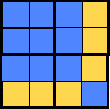
\includegraphics[width=0.19\textwidth]{signs}
                \end{center}
                \caption{The signs associated with a wavelet coefficient. Blue is positive and orange is negative; both magnitudes are one.  }
                \label{fig:signs}    
            \end{wrapfigure}

        \subsection{The approximation algorithm}
            I went through a long, intensive process to find this. But of course, there's a simple mathematical fix to this problem. Let's say you have 
                $$AXB = C$$
                Using the \href{\kron}{Kroneker product} ($\otimes$), that's equivalent to

                $$(B^T \otimes A)\text{vec}(X) = \text{vec}(C) = \text{vec}(AXB) $$

                This is remarkably similar to the 1D case. You have to delete the rows corresponding to where the finer detail lies and the columns that correspond to where you don't sample.

                In our case, we have $w = c x r$, where $c$ performs the complete wavelet transform on the columns and $r$ the complete transform on the rows. 

                \subsubsection{Scaling}
                    We are currently saying ``we're interested in these coefficients, and don't care where they lie.'' That means that to get an accurate reconstruction, we have to have scale our function right.

                    But, we could just approximate our wavelet to some level. Then, when we don't care about terms, they're automatically set to 0 (via the dot product).


        \subsection{Which indices are important?}
            Initially, I thought that the wavelet transform had to be recursive. That makes it really tricky for the indices -- you would have to make \texttt{dwt\_ind} functions, and keep doing it. 

            But after I talked to Ashkay, I learned that you can do the full wavelet transform on each row then each wavelet transform on each column. That makes this function trivial: it's just a matter of indexing. 

        \subsection{The reconstruction}
            In the wavelet domain, we have a tree that corresponds to the image. An example is in \Cref{fig:tree}. The upper levels of the tree represent the lower frequency terms. Since there's no need to closely sample a low frequency term, we only sample where there are high frequencies. 

            We know that if any of these ``branches'' are close enough to zero ($|x| < \lambda$) that all of it's child branches are close enough to 0 as well. Therefore, we only look at where the branches are not close enough to zero ($|x| > \lambda$). As we go further down the branch, we form a better approximation of the wavelet transform.
            
            \begin{figure}[h]
                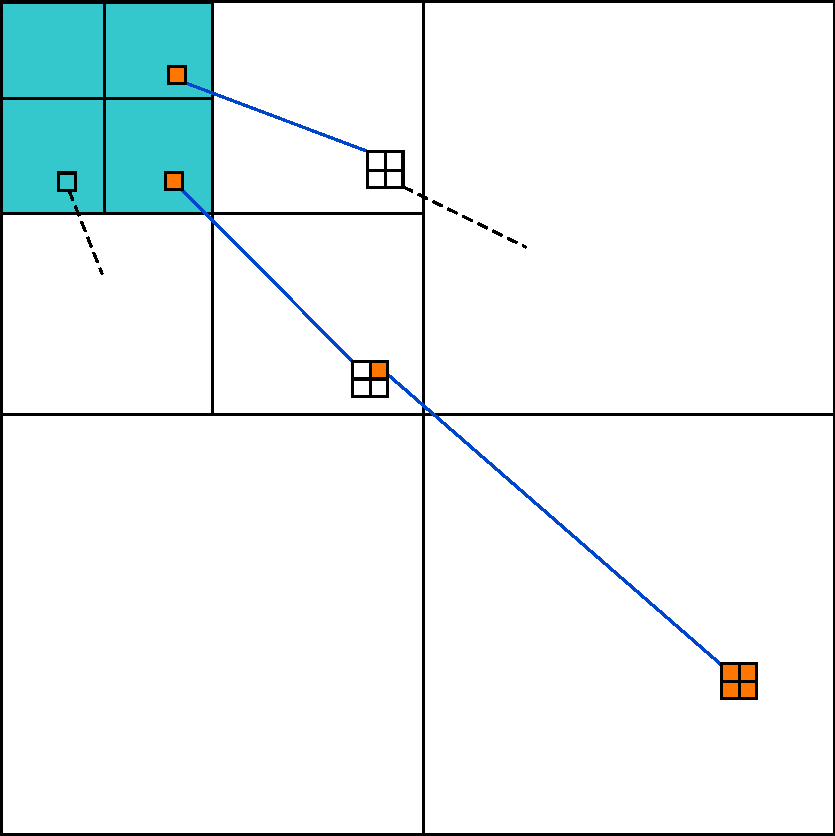
\includegraphics[angle=0]{better_diagram}
                \caption{A visualization of our tree. The blue square is our current node. Only two of it's components are non-zero, meaning that there's more detail at lower levels we need to look at closer. We then build a better and better approximation as we need too.}
                \label{fig:tree}
            \end{figure}
            
            Where we choose to look (or where we sample) is near the edges. The wavelet transform is zero for a constant: it has no high frequency terms.




            \bibliographystyle{plain}
            \bibliography{BibDesk}
            \printbibliography{}

\end{document}





































